\documentclass{article}
\usepackage{graphicx}
\usepackage{listings}
\usepackage{color}
\usepackage{amsmath}
\usepackage{amsfonts}
\usepackage{bm}
\usepackage[utf8]{inputenc}

\title{Modelli geometrici\\
	Corso di LSMC, a.a. 2017-2018}
\author{Davide Gori\\
	550282}


\definecolor{backcolour}{rgb}{0.95,0.95,0.92}
\definecolor{gray}{rgb}{0.5,0.5,0.5}
\lstset{basicstyle=\ttfamily\small,
	columns=fullflexible,
	numbers=left,
	numberstyle=\tiny\ttfamily\color{gray},
	backgroundcolor=\color{backcolour},
	tabsize=4,
	language=Octave
}


\begin{document}
	\maketitle
	\section{Prima sperimentazione: curva clotoide}
	Si consideri la curva (clotoide) definita dalle equazioni:
	\begin{equation}
	\begin{cases}
	y'=\cos(x^2) \\
	z'=\sin(x^2) \\
	y(0)=0\\
	z(0)=0
	\end{cases}
	\end{equation}
	Disegnerò la clotoide per $x>0$ e per $x<0$, verificandone eventuali simmetrie. Stimando le coordinate dei punti asintotici facendo variare $x$ in intervalli molto ampi.
	\subsection{Il codice}
	Questo è lo script che realizza la sperimentazione:
	\lstinputlisting{LabSper_7_1.m}
	\subsection{Risultati}
	Riportiamo i grafici in output.\\
	Notiamo che le equazioni sono invarianti per cambio di segno di $x$. Le due curve sono simmetriche rispetto al punto medio del segmento che congiunge i due estremi della curva. In particolare graficamente si osserva che i due estremi sono circa $(0,0)$ e $(0.625, 0.625)$.
	\begin{figure}[htp!]
		\centering 
		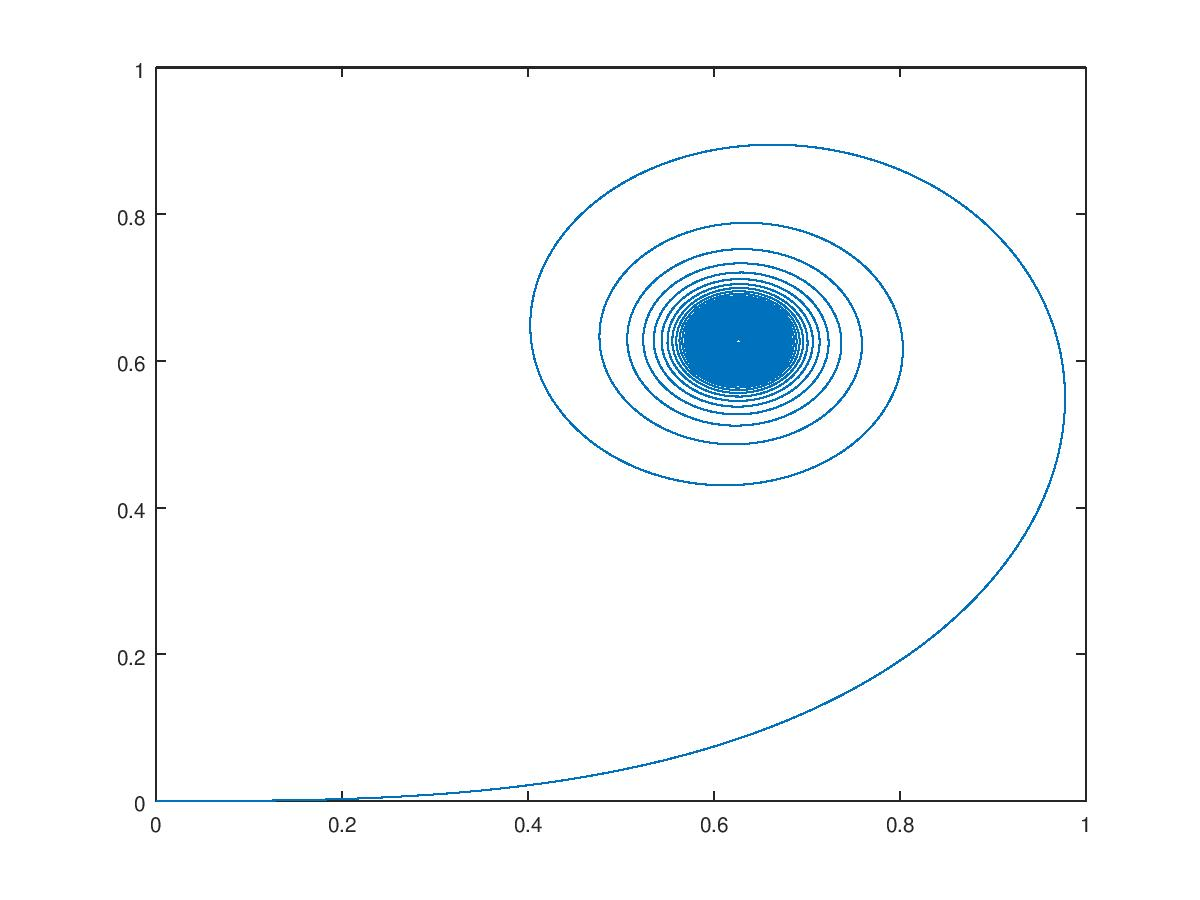
\includegraphics[width=\textwidth]{7_1_a.jpeg}
	\end{figure}
	\begin{figure}[htp!]
		\centering 
		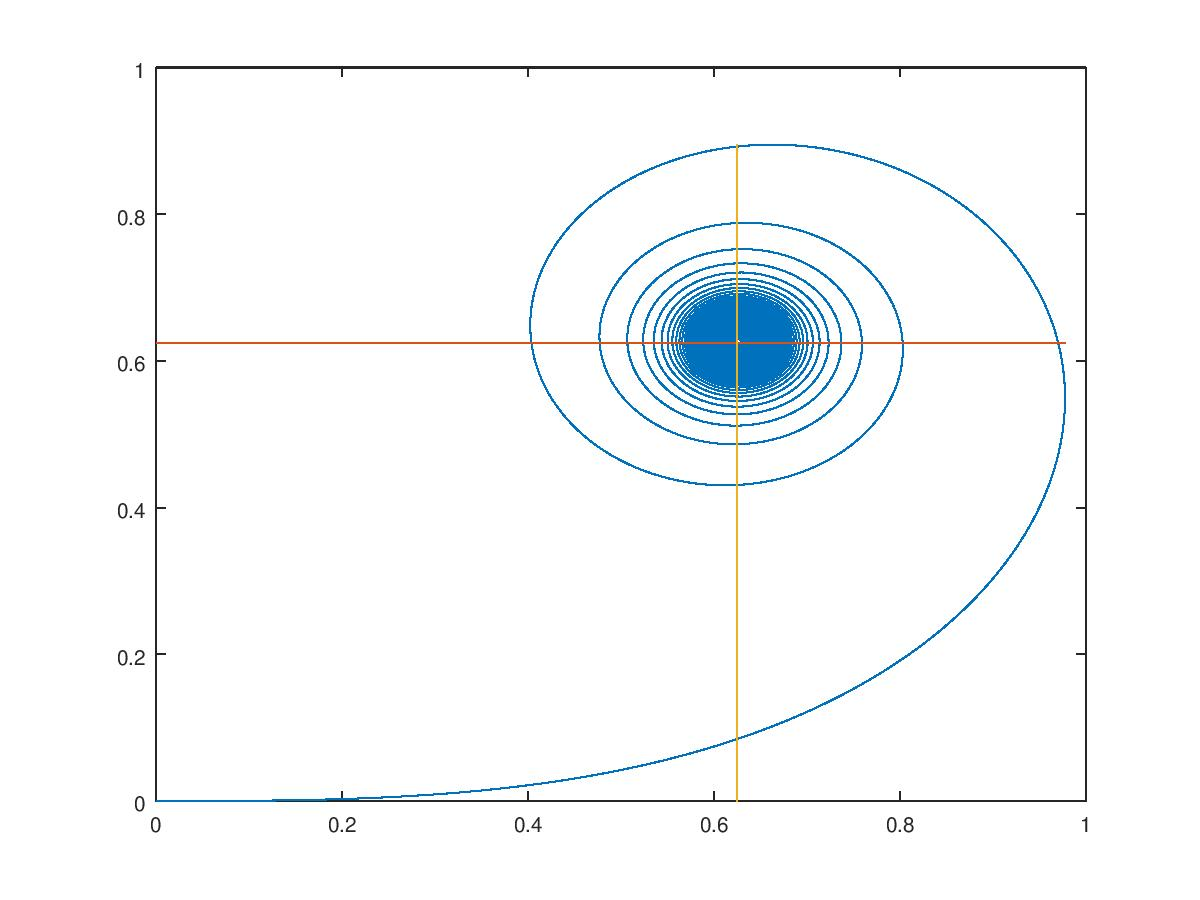
\includegraphics[width=\textwidth]{7_1_a_bis.jpeg}
	\end{figure}
	\begin{figure}[htp!]
		\centering 
		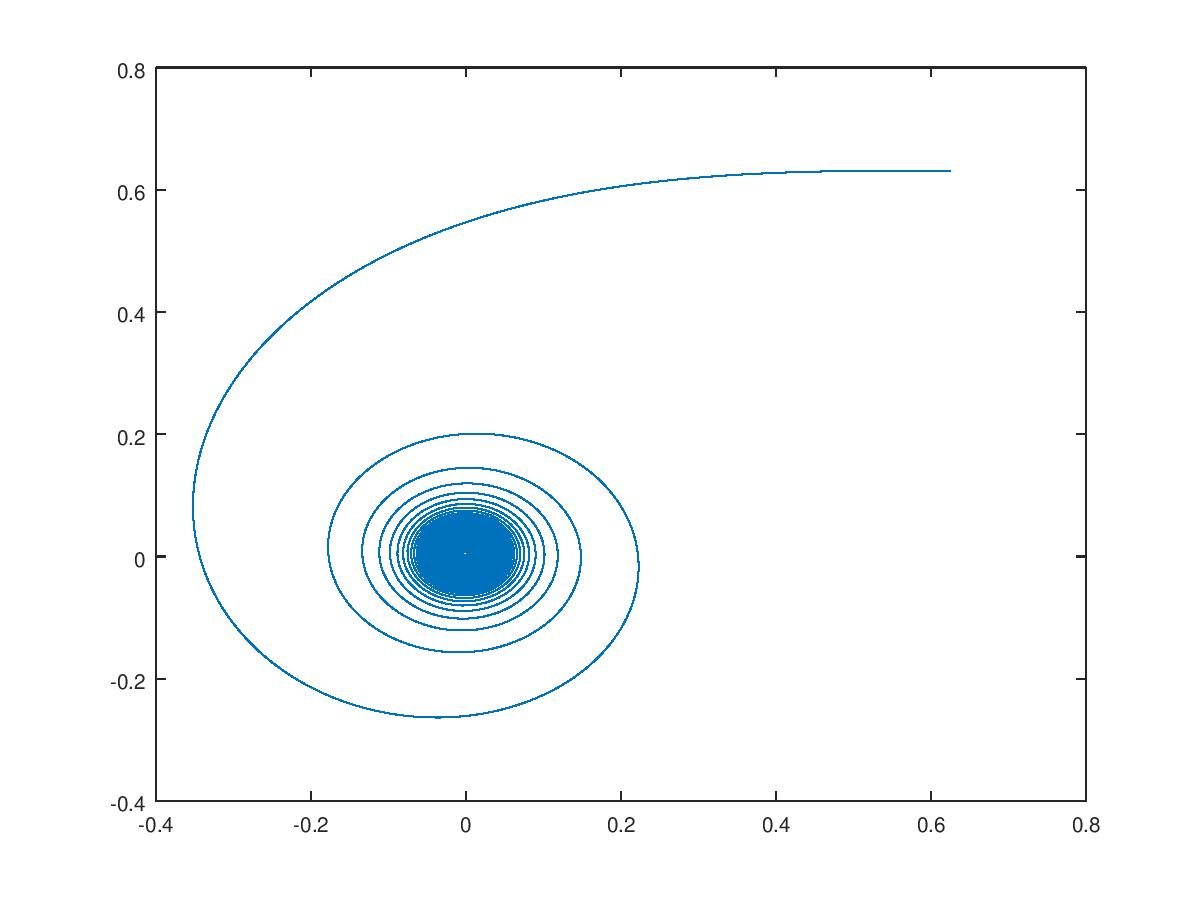
\includegraphics[width=\textwidth]{7_1_b.jpeg}
	\end{figure}
	\newpage
	\section{Seconda sperimentazione: spirale logaritmica}
	Si consideri la curva di equazioni parametriche:
	\begin{equation}
	\begin{cases}
	x(\theta)=ab^\theta \cos(\theta) \\
	y(\theta)=ab^\theta \sin(\theta) \\
	\end{cases}
	\end{equation}
	Tale curva è nota come spirale logaritmica.\\
	Determinerò un problema ai valori iniziali che definisca tale curva e, fissati i dati, lo risolverò numericamente mediante la routine {\tt ode45}. Traccerò quindi il grafico della spirale logaritmica corrispondente usando i due metodi (equazioni parametriche e soluzione del problema differenziale).\\
	\subsection{Il codice}
	Derivando si ottiene $[x(\theta), y(\theta)]=[a \ln(b) y, a \ln(b) x]$.
	Questo è lo script che realizza la sperimentazione:
	\lstinputlisting{LabSper_7_2.m}
	
	\subsection{Risultati}
	Riporto il grafico in output.\\
	\begin{figure}[htp!]
		\centering 
		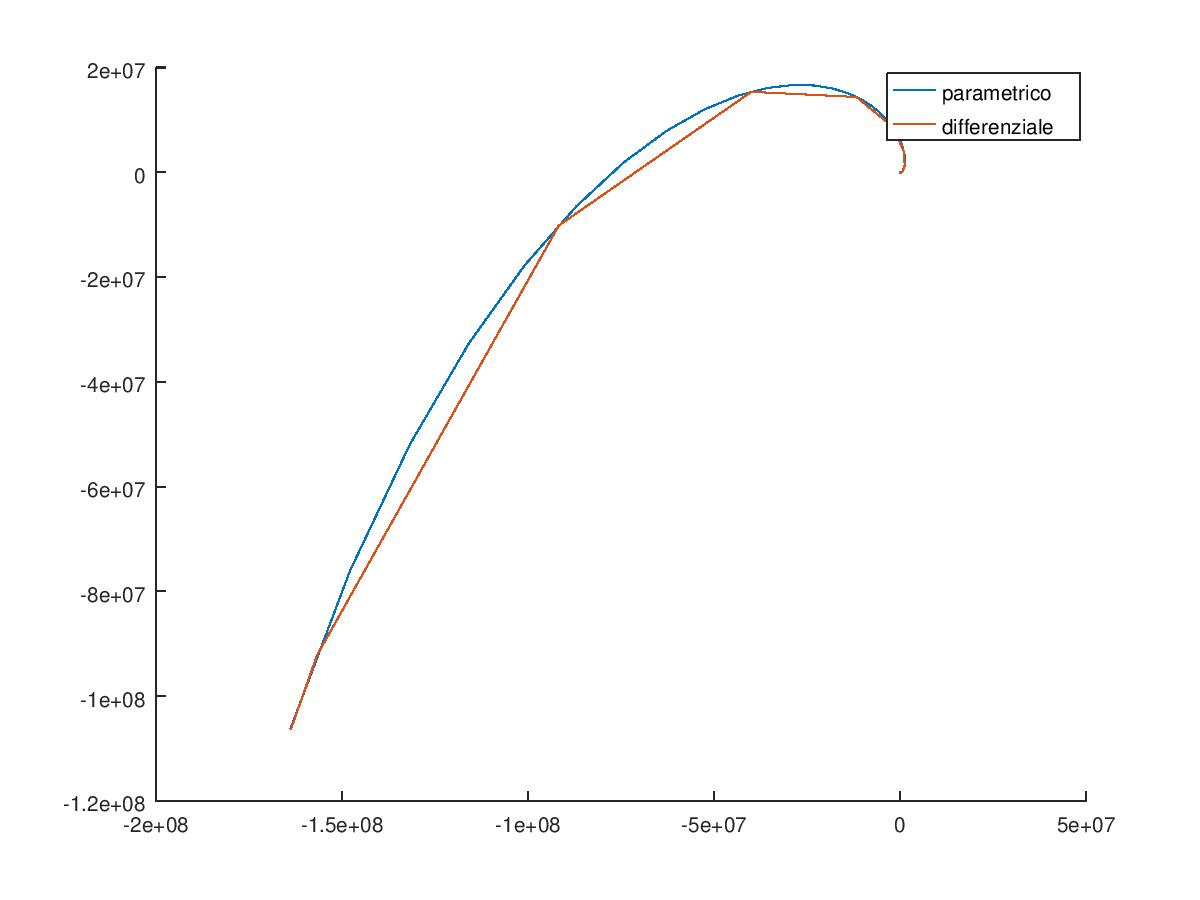
\includegraphics[width=\textwidth]{7_2.jpeg}
	\end{figure}
\end{document}